\RequirePackage{silence}
\WarningFilter{biblatex}{Patching footnotes failed}
%\documentclass[10pt, compress,british,xcolor={svgnames,dvipsnames,x11names},trans]{beamer}

\documentclass[t,10pt,numbers,fleqn,usenames,xcolor=dvipsnames]{beamer}
%\usetheme{Frankfurt}
%\usetheme{Montpellier}
%\usecolortheme{seahorse}
%\useinnertheme{rectangles}
%\usetheme{warsaw}
%\usepackage[show]{ed}
\usepackage{template}
\usepackage{graphicx}
%\usepackage{subcaption}
\usepackage{verbatim}
\usepackage{amsfonts}
\usepackage{amsmath}
\usepackage{stmaryrd}
\usepackage{listings}
\lstset{basicstyle={\ttfamily\footnotesize}}
\usepackage{pgf}
\usepackage{pgfpages} 
\usepackage{tikz}
\usetikzlibrary{tikzmark}
\usepackage{tikz-cd}
\usetikzlibrary{cd}
\usepackage{upgreek}
%\usepackage[english]{babel}
\usepackage{adjustbox}
%\usepackage[dvipsnames]{xcolor}
\usepackage{wrapfig}
\usepackage{tcolorbox}

\usepackage{../style_files/macros}

%\usepackage[hyphens]{url}
%\usepackage[colorlinks=true]{hyperref}

\mode<presentation>{}
\setbeamertemplate{footline}[frame number]

\usepackage{minted}

%\AtBeginSection[]
%{
%    \begin{frame}<beamer>
%    \frametitle{Outline for section \thesection}
%    \tableofcontents[currentsection]
%\end{frame}
%}


\usepackage{xkeyval}
%\usepackage{todonotes}
%\presetkeys{todonotes}{inline}{}

\setlength{\arrayrulewidth}{0.5mm}
\setlength{\tabcolsep}{18pt}
\renewcommand{\arraystretch}{1.5}
\usepackage{color}
\hypersetup{colorlinks=false,
    urlcolor=blue, 
    linkcolor=white,
    citecolor=blue,
    unicode=false, 
}


%\usepackage{../../2019/Presentation/macros}
%\usepackage{../../2019/Presentation/local}
%\usepackage{../../2019/Presentation/basics}

\DeclareUnicodeCharacter{25AE}{\^proofend}

\makeatletter
\setlength{\@fptop}{0pt}
\makeatother

\definecolor{carriercolor}{rgb}{0.0,0.5,1.00}
%\definecolor{equivcolor}{rgb}{Plum}
%\definecolor{hiercolor}{rgb}{}
\definecolor{ourblue}{rgb}{0.90,0.98,1.0}
\definecolor{ourpink}{rgb}{1.0,0.96,0.99}
\definecolor{ultramarine}{rgb}{0, 0.125, 0.376}
\newcommand{\tog}{tog}
\newcommand{\etc}{etc.}
%\newcommand{\equivEmph}[1]{\textbf{#1}}
\newcommand{\equivEmph}[1]{\textcolor{Plum}{\textbf{\text{#1}}}}
\newcommand{\hierarchEmph}[1]{{\textcolor{Plum}{\textbf{\text{#1}}}}}

\title{Leveraging Information Contained in Theory Presentations}
%\institute{\vspace{.5cm} McMaster University}
\author{\textbf{Yasmine Sharoda} \newline 
\newline \underline{\textit{Supervisors:}} \vspace{0.5em}\\ 
Jacques Carette and William M. Farmer} 
%\institute{McMaster University}
\date{}
\titlegraphic{
\hspace*{8cm}
\includegraphics[width=2cm]{figures/mac-logo.png}
}


\begin{document}
    
\frame{\titlepage}
%\section{Motivation and Problem}

%\plain{A large library of Mathematics is \newline
%\textcolor{Orange}{\emph{useful}} but \textcolor{Orange}{\emph{hard to build}}} 

\begin{frame}[fragile] 
\frametitle{Large Libraries of Mathematics}
% The quest for a large library of Mathematics
%\begin{center}
%A large library of Mathematics is \textcolor{Orange}{\textbf{useful}} %but hard to build
%\end{center}
%\vfill 
\begin{itemize}
\item QED Manifesto, 1994: 
\begin{itemize}
\item One library to formalize all of Mathematics 
\end{itemize}
\vspace{0.3cm}
%\item Universal Digital Math Library, 2004: 
%\begin{itemize}
%\item Heterogeneous, Interconnecting libraries.  
%\end{itemize}
\pause
\item Building a library requires: 
\begin{itemize}
\item Foundation 
\item Organizational Structures 
\item ... 
\item Huge amount of knowledge $\Rightarrow$ \textbf{Labour Intensive} 
\end{itemize}
\end{itemize}
\vfill 
\pause 
Current libraries of mathematics are full of \textcolor{Orange}{\textbf{\emph{redundancy}}}
\end{frame}

\begin{comment}
\begin{frame}
\frametitle{Monoid Definition} 
A monoid is a triple $(M,p,1)$ in which: 
\begin{itemize}
\item $M$ is a non-empty set. 
\item $p$ is an associative binary composition (or product) in $M$. 
\item $1$ is an element of $M$ such that: \\
$p(1,a)= a = p(a,1)$ for all $a \in M$.
\end{itemize}
\end{frame}
\end{comment}

\begin{frame}[fragile]
\frametitle{Monoid: One theory, Multiple Representations} 
\begin{onlyenv}<1>
\begin{figure}
  \scalebox{.95}{\footnotesize
\begin{adjustbox}{width=1.2\columnwidth,center}
\begin{tabular}{p{7cm} p{7cm} p{7cm}}  
\underline{Lean}
\begin{minted}[mathescape=true, escapeinside=||]{lean} 
class monoid (M : Type u)
 extends semigroup M, has|$\_$|one M :=
  (one_mul : |$\forall$| a : M, 1 * a = a) 
  (mul_one : |$\forall$| a : M, a * 1 = a)   
\end{minted} 
\vspace{0.5cm}
\underline{MMT}
\begin{minted}[mathescape=true, escapeinside=~~]{coq}
theory Monoid : ~$?$~NatDed = 
 includes ~$?$~Semigroup 
 unit : tm u ~$\#$~ e 
 unit_axiom : ~$\vdash$~ ~$\forall$~ [x] = x * e = x    
 
theory Semigroup : ~$?$~NatDed = 
 u : sort 
 comp : tm u ~$\to$~ tm u ~$\to$~ tm u 
  ~$\#$~ 1 * 2 prec 40
 assoc : ~$\vdash$~ ~$\forall$~ [x, y, z]
  (x * y) * z = x * (y * z)    
 assocLeftToRight : 
  {x,y,z} ~$\vdash$~ (x * y) * z 
          = x * (y * z) 
  = [x,y,z] 
   allE (allE (allE assoc x) y) z
 assocRightToLeft : 
  {x,y,z} ~$\vdash$~  x * (y * z) 
           = (x * y) * z 
  = [x,y,z] sym assocLR    
\end{minted}     
&
\underline{Haskell}
\begin{minted}[mathescape, escapeinside=~~]{haskell}
class Semigroup a => Monoid a where 
  mempty :: a 
  mappend :: a -> a -> a 
  mappend = (<>) 
  mconcat :: [a] -> a 
  mconcat = foldr mappend mempty 
\end{minted} 
\vspace{0.5cm}
\underline{Coq}
\begin{minted}[mathescape=true, escapeinside=~~]{coq}
class Monoid {A : type}
 (dot : A ~$\to$~ A ~$\to$~ A)
 (one : A) : Prop := {
  dot_assoc : 
   forall x y z : A, 
   (dot x (dot y z)) = dot (dot x y) z
  unit_left  : forall x, dot one x = x 
  unit_right : forall x, dot x one = x              
}
~$\text{\textit{Alternative Definition:}}$~
Record monoid := {
 dom : Type; 
 op : dom -> dom -> dom 
  where "x * y" := op x y; 
 id : dom where "1" := id; 
 assoc : forall x y z, x * (y * z) = (x * y) * z; 
 left_neutral : forall x, 1 * x = x; 
 right_neutal : forall x, x * 1 = x; 
}
\end{minted} 
&
\underline{Agda}
\begin{minted}[mathescape=true, escapeinside=~~]{agda} 
record Monoid c ~$\ell$~ : Set (suc (c ~$\sqcup$~ ~$\ell$~)) where 
 infixl 7 _~$\bullet$~_
 infix 4 _~$\approx$~_
 field 
  Carrier : Set c 
  _~$\approx$~_ : Rel Carrier ~$\ell$~ 
  _~$\bullet$~_ : Op~$_2$~ Carrier 
  isMonoid : IsMonoid _~$\approx$~_ _~$\bullet$~_ ~$\varepsilon$~ 
  
record IsMonoid (~$\bullet$~ : Op~$_2$~) (~$\varepsilon$~ : A) 
: Set (a ~$\sqcup$~ ~$\ell$~) where 
  field 
   isSemigroup : IsSemigroup ~$\bullet$~ 
   identity : Identity ~$\varepsilon$~ 
       
   open IsSemigroup isSemigroup public 
   
   identity~$^l$~ : LeftIdentity ~$\varepsilon$~ ~$\bullet$~ 
   identity~$^l$~ = proj~$_1$~ identity 
   identity~$^r$~ : Rightdentity ~$\varepsilon$~ ~$\bullet$~ 
   identity~$^r$~ = proj~$_2$~ identity        
\end{minted}       
\end{tabular}  
\end{adjustbox}
}
\end{figure}
\end{onlyenv}
\begin{onlyenv}<2>
\begin{figure}
  \scalebox{.95}{\footnotesize
\begin{adjustbox}{width=1.2\columnwidth,center}
\begin{tabular}{p{7cm} p{7cm} p{7cm}}  
\underline{Lean}
\begin{minted}[mathescape=true, escapeinside=||]{lean} 
class monoid (M : Type u)
 |\fcolorbox{red}{white}{extends semigroup M, has$\_$one M}| :=
  (one_mul : |$\forall$| a : M, 1 * a = a) 
  (mul_one : |$\forall$| a : M, a * 1 = a)   
\end{minted} 
\vspace{0.5cm}
\underline{MMT}
\begin{minted}[mathescape=true, escapeinside=~~]{coq}
theory Monoid : ~$?$~NatDed = 
 ~\fcolorbox{red}{white}{includes $?$Semigroup}~ 
 unit : tm u ~$\#$~ e 
 unit_axiom : ~$\vdash$~ ~$\forall$~ [x] = x * e = x    
 
theory Semigroup : ~$?$~NatDed = 
 u : sort 
 comp : tm u ~$\to$~ tm u ~$\to$~ tm u 
  ~$\#$~ 1 * 2 prec 40
 assoc : ~$\vdash$~ ~$\forall$~ [x, y, z]
  (x * y) * z = x * (y * z)    
 assocLeftToRight : 
  {x,y,z} ~$\vdash$~ (x * y) * z 
          = x * (y * z) 
  = [x,y,z] 
   allE (allE (allE assoc x) y) z
 assocRightToLeft : 
  {x,y,z} ~$\vdash$~  x * (y * z) 
           = (x * y) * z 
  = [x,y,z] sym assocLR    
\end{minted}     
&
\underline{Haskell}
\begin{minted}[mathescape, escapeinside=~~]{haskell}
class ~\fcolorbox{red}{white}{Semigroup a => Monoid a}~ where 
  mempty :: a 
  mappend :: a -> a -> a 
  mappend = (<>) 
  mconcat :: [a] -> a 
  mconcat = foldr mappend mempty 
\end{minted} 
\vspace{0.5cm}
\underline{Coq}
\begin{minted}[mathescape=true, escapeinside=~~]{coq}
class Monoid {A : type}
 (dot : A ~$\to$~ A ~$\to$~ A)
 (one : A) : Prop := {
  dot_assoc : 
   forall x y z : A, 
   (dot x (dot y z)) = dot (dot x y) z
  unit_left  : forall x, dot one x = x 
  unit_right : forall x, dot x one = x              
}
~$\text{\textit{Alternative Definition:}}$~
Record monoid := {
 dom : Type; 
 op : dom -> dom -> dom 
  where "x * y" := op x y; 
 id : dom where "1" := id; 
 assoc : forall x y z, x * (y * z) = (x * y) * z; 
 left_neutral : forall x, 1 * x = x; 
 right_neutal : forall x, x * 1 = x; 
}
\end{minted} 
&
\underline{Agda}
\begin{minted}[mathescape=true, escapeinside=~~]{agda} 
record Monoid c ~$\ell$~ : Set (suc (c ~$\sqcup$~ ~$\ell$~)) where 
 infixl 7 _~$\bullet$~_
 infix 4 _~$\approx$~_
 field 
  Carrier : Set c 
  _~$\approx$~_ : Rel Carrier ~$\ell$~ 
  _~$\bullet$~_ : Op~$_2$~ Carrier 
  isMonoid : IsMonoid _~$\approx$~_ _~$\bullet$~_ ~$\varepsilon$~ 
  
record IsMonid (~$\bullet$~ : Op~$_2$~) (~$\varepsilon$~ : A) 
: Set (a ~$\sqcup$~ ~$\ell$~) where 
  field 
   isSemiring : IsSemiring ~$\bullet$~ 
   identity : Identity ~$\varepsilon$~ 
       
   open IsSemigroup isSemigroup public 
   
   identity~$^l$~ : LeftIdentity ~$\varepsilon$~ ~$\bullet$~ 
   identity~$^l$~ = proj~$_1$~ identity 
   identity~$^r$~ : Rightdentity ~$\varepsilon$~ ~$\bullet$~ 
   identity~$^r$~ = proj~$_2$~ identity        
\end{minted}       
\end{tabular}  
\end{adjustbox}
}
\end{figure}
\end{onlyenv}
\begin{onlyenv}<3>
\begin{figure}
  \scalebox{.95}{\footnotesize
\begin{adjustbox}{width=1.2\columnwidth,center}
\begin{tabular}{p{7cm} p{7cm} p{7cm}}  
\underline{Lean}
\begin{minted}[mathescape=true, escapeinside=||]{lean} 
class monoid |\fcolorbox{red}{white}{(M : Type u)}|
 extends semigroup M, has|$\_$|one M :=
  (one_mul : |$\forall$| a : M, 1 * a = a) 
  (mul_one : |$\forall$| a : M, a * 1 = a)   
\end{minted} 
\vspace{0.5cm}
\underline{MMT}
\begin{minted}[mathescape=true, escapeinside=~~]{coq}
theory Monoid : ~$?$~NatDed = 
 includes ~$?$~Semigroup 
 unit : tm u ~$\#$~ e 
 unit_axiom : ~$\vdash$~ ~$\forall$~ [x] = x * e = x    
 
theory Semigroup : ~$?$~NatDed = 
 u : sort 
 comp : tm u ~$\to$~ tm u ~$\to$~ tm u 
  ~$\#$~ 1 * 2 prec 40
 assoc : ~$\vdash$~ ~$\forall$~ [x, y, z]
  (x * y) * z = x * (y * z)    
 assocLeftToRight : 
  {x,y,z} ~$\vdash$~ (x * y) * z 
          = x * (y * z) 
  = [x,y,z] 
   allE (allE (allE assoc x) y) z
 assocRightToLeft : 
  {x,y,z} ~$\vdash$~  x * (y * z) 
           = (x * y) * z 
  = [x,y,z] sym assocLR    
\end{minted}     
&
\underline{Haskell}
\begin{minted}[mathescape, escapeinside=~~]{haskell}
class Semigroup a => Monoid ~\fcolorbox{red}{white}{a}~ where 
  mempty :: a 
  mappend :: a -> a -> a 
  mappend = (<>) 
  mconcat :: [a] -> a 
  mconcat = foldr mappend mempty 
\end{minted} 
\vspace{0.5cm}
\underline{Coq}
\begin{minted}[mathescape=true, escapeinside=~~]{coq}
class Monoid ~\fcolorbox{red}{white}{{A : type}}~
 ~\fcolorbox{red}{white}{(dot : A $\to$ A $\to$ A)}~
 ~\fcolorbox{red}{white}{(one : A)}~ : Prop := {
  dot_assoc : 
   forall x y z : A, 
   (dot x (dot y z)) = dot (dot x y) z
  unit_left  : forall x, dot one x = x 
  unit_right : forall x, dot x one = x              
}
~$\text{\textit{Alternative Definition:}}$~
Record monoid := {
 dom : Type; 
 op : dom -> dom -> dom 
  where "x * y" := op x y; 
 id : dom where "1" := id; 
 assoc : forall x y z, x * (y * z) = (x * y) * z; 
 left_neutral : forall x, 1 * x = x; 
 right_neutal : forall x, x * 1 = x; 
}
\end{minted} 
&
\underline{Agda}
\begin{minted}[mathescape=true, escapeinside=~~]{agda} 
record Monoid c ~$\ell$~ : Set (suc (c ~$\sqcup$~ ~$\ell$~)) where 
 infixl 7 _~$\bullet$~_
 infix 4 _~$\approx$~_
 field 
  Carrier : Set c 
  _~$\approx$~_ : Rel Carrier ~$\ell$~ 
  _~$\bullet$~_ : Op~$_2$~ Carrier 
  isMonoid : IsMonoid _~$\approx$~_ _~$\bullet$~_ ~$\varepsilon$~ 
  
record IsMonid ~\fcolorbox{red}{white}{($\bullet$ : Op$_2$) ($\varepsilon$ : A)}~ 
: Set (a ~$\sqcup$~ ~$\ell$~) where 
  field 
   isSemiring : IsSemiring ~$\bullet$~ 
   identity : Identity ~$\varepsilon$~ 
       
   open IsSemigroup isSemigroup public 
   
   identity~$^l$~ : LeftIdentity ~$\varepsilon$~ ~$\bullet$~ 
   identity~$^l$~ = proj~$_1$~ identity 
   identity~$^r$~ : Rightdentity ~$\varepsilon$~ ~$\bullet$~ 
   identity~$^r$~ = proj~$_2$~ identity        
\end{minted}       
\end{tabular}  
\end{adjustbox}
}
\end{figure}
\end{onlyenv}
\begin{onlyenv}<4>
\begin{figure}
  \scalebox{.95}{\footnotesize
\begin{adjustbox}{width=1.2\columnwidth,center}
\begin{tabular}{p{7cm} p{7cm} p{7cm}}  
\underline{Lean}
\begin{minted}[mathescape=true, escapeinside=||]{lean} 
class monoid (M : Type u)
 extends semigroup M, has|$\_$|one M :=
  (one_mul : |$\forall$| a : M, 1 * a = a) 
  (mul_one : |$\forall$| a : M, a * 1 = a)   
\end{minted} 
\vspace{0.5cm}
\underline{MMT}
\begin{minted}[mathescape=true, escapeinside=~~]{coq}
theory Monoid : ~$?$~NatDed = 
 includes ~$?$~Semigroup 
 unit : tm u ~$\#$~ e 
 unit_axiom : ~$\vdash$~ ~$\forall$~ [x] = x * e = x    
 
theory Semigroup : ~$?$~NatDed = 
 u : sort 
 comp : tm u ~$\to$~ tm u ~$\to$~ tm u 
  ~$\#$~ 1 * 2 prec 40
 assoc : ~$\vdash$~ ~$\forall$~ [x, y, z]
  (x * y) * z = x * (y * z)    
 assocLeftToRight : 
  {x,y,z} ~$\vdash$~ (x * y) * z 
          = x * (y * z) 
  = [x,y,z] 
   allE (allE (allE assoc x) y) z
 assocRightToLeft : 
  {x,y,z} ~$\vdash$~  x * (y * z) 
           = (x * y) * z 
  = [x,y,z] sym assocLR    
\end{minted}     
&
\underline{Haskell}
\begin{minted}[mathescape, escapeinside=~~]{haskell}
class Semigroup a => Monoid a where 
  mempty :: a 
  mappend :: a -> a -> a 
  mappend = (<>) 
  mconcat :: [a] -> a 
  mconcat = foldr mappend mempty 
\end{minted} 
\vspace{0.5cm}
\underline{Coq}
\begin{minted}[mathescape=true, escapeinside=~~]{coq}
class Monoid {A : type}
 (dot : A ~$\to$~ A ~$\to$~ A)
 (one : A) : Prop := {
  dot_assoc : 
   forall x y z : A, 
   (dot x (dot y z)) = dot (dot x y) z
  unit_left  : forall x, dot one x = x 
  unit_right : forall x, dot x one = x              
}
~$\text{\textit{Alternative Definition:}}$~
Record monoid := {
 dom : Type; 
 op : dom -> dom -> dom 
  where "x * y" := op x y; 
 id : dom where "1" := id; 
 assoc : forall x y z, x * (y * z) = (x * y) * z; 
 left_neutral : forall x, 1 * x = x; 
 right_neutal : forall x, x * 1 = x; 
}
\end{minted} 
&
\underline{Agda}
\begin{minted}[mathescape=true, escapeinside=~~]{agda} 
record Monoid c ~$\ell$~ : Set (suc (c ~$\sqcup$~ ~$\ell$~)) where 
 infixl 7 _~$\bullet$~_
 infix 4 _~$\approx$~_
 field 
  Carrier : Set c 
  ~\fcolorbox{red}{white}{\_$\approx$\_ : Rel Carrier $\ell$}~ 
  _~$\bullet$~_ : Op~$_2$~ Carrier 
  isMonoid : IsMonoid _~$\approx$~_ _~$\bullet$~_ ~$\varepsilon$~ 
  
record IsMonoid (~$\bullet$~ : Op~$_2$~) (~$\varepsilon$~ : A) 
: Set (a ~$\sqcup$~ ~$\ell$~) where 
  field 
   isSemigroup : IsSemigroup ~$\bullet$~ 
   identity : Identity ~$\varepsilon$~ 
       
   open IsSemigroup isSemigroup public 
   
   identity~$^l$~ : LeftIdentity ~$\varepsilon$~ ~$\bullet$~ 
   identity~$^l$~ = proj~$_1$~ identity 
   identity~$^r$~ : Rightdentity ~$\varepsilon$~ ~$\bullet$~ 
   identity~$^r$~ = proj~$_2$~ identity        
\end{minted}       
\end{tabular}  
\end{adjustbox}
}
\end{figure}
\end{onlyenv}
\begin{onlyenv}<5>
\begin{figure}
  \scalebox{.95}{\footnotesize
\begin{adjustbox}{width=1.2\columnwidth,center}
\begin{tabular}{p{7cm} p{7cm} p{7cm}}  
\underline{Lean}
\begin{minted}[mathescape=true, escapeinside=||]{lean} 
class monoid (M : Type u)
 extends semigroup M, has|$\_$|one M :=
  (one_mul : |$\forall$| a : M, 1 * a = a) 
  (mul_one : |$\forall$| a : M, a * 1 = a)   
\end{minted} 
\vspace{0.5cm}
\underline{MMT}
\begin{minted}[mathescape=true, escapeinside=~~]{coq}
theory Monoid : ~$?$~NatDed = 
 includes ~$?$~Semigroup 
 unit : tm u ~$\#$~ e 
 unit_axiom : ~$\vdash$~ ~$\forall$~ [x] = x * e = x    
 
theory Semigroup : ~$?$~NatDed = 
 u : sort 
 comp : tm u ~$\to$~ tm u ~$\to$~ tm u 
  ~$\#$~ 1 * 2 prec 40
 assoc : ~$\vdash$~ ~$\forall$~ [x, y, z]
  (x * y) * z = x * (y * z)    
 assocLeftToRight : 
  {x,y,z} ~$\vdash$~ (x * y) * z 
          = x * (y * z) 
  = [x,y,z] 
   allE (allE (allE assoc x) y) z
 assocRightToLeft : 
  {x,y,z} ~$\vdash$~  x * (y * z) 
           = (x * y) * z 
  = [x,y,z] sym assocLR    
\end{minted}     
&
\underline{Haskell}
\begin{minted}[mathescape, escapeinside=~~]{haskell}
class Semigroup a => Monoid a where 
  mempty :: a 
  mappend :: a -> a -> a 
  mappend = (<>) 
  mconcat :: [a] -> a 
  mconcat = foldr mappend mempty 
\end{minted} 
\vspace{0.5cm}
\underline{Coq}
\begin{minted}[mathescape=true, escapeinside=~~]{coq}
class Monoid {A : type}
 (dot : A ~$\to$~ A ~$\to$~ A)
 (one : A) : Prop := {
  dot_assoc : 
   forall x y z : A, 
   (dot x (dot y z)) = dot (dot x y) z
  unit_left  : forall x, dot one x = x 
  unit_right : forall x, dot x one = x              
}
~$\text{\textit{Alternative Definition:}}$~
Record monoid := {
 dom : Type; 
 op : dom -> dom -> dom 
  where "x * y" := op x y; 
 id : dom where "1" := id; 
 assoc : forall x y z, x * (y * z) = (x * y) * z; 
 left_neutral : forall x, 1 * x = x; 
 right_neutal : forall x, x * 1 = x; 
}
\end{minted} 
&
\underline{Agda}
\begin{minted}[mathescape=true, escapeinside=~~]{agda} 
record Monoid c ~$\ell$~ : Set (suc (c ~$\sqcup$~ ~$\ell$~)) where 
 infixl 7 _~$\bullet$~_
 infix 4 _~$\approx$~_
 field 
  Carrier : Set c 
  ~\fcolorbox{red}{white}{\_$\approx$\_ : Rel Carrier $\ell$}~ 
  _~$\bullet$~_ : Op~$_2$~ Carrier 
  isMonoid : IsMonoid _~$\approx$~_ _~$\bullet$~_ ~$\varepsilon$~ 
  
record IsMonoid (~$\bullet$~ : Op~$_2$~) (~$\varepsilon$~ : A) 
: Set (a ~$\sqcup$~ ~$\ell$~) where 
  field 
   isSemigroup : IsSemigroup ~$\bullet$~ 
   identity : Identity ~$\varepsilon$~ 
       
   open IsSemigroup isSemigroup public 
   
   identity~$^l$~ : LeftIdentity ~$\varepsilon$~ ~$\bullet$~ 
   identity~$^l$~ = proj~$_1$~ identity 
   identity~$^r$~ : Rightdentity ~$\varepsilon$~ ~$\bullet$~ 
   identity~$^r$~ = proj~$_2$~ identity        
\end{minted}       
\end{tabular}  
\end{adjustbox}
}
\end{figure}
\pause
Can we abstract over these design decisions? 
\end{onlyenv}
\end{frame}

\begin{frame}[fragile] 
\frametitle{Monoid: One theory, Many Constructions} 
\begin{columns}
    \begin{column}{0.45\textwidth}
\begin{minted}[escapeinside=||,mathescape=true,fontsize=\tiny]{agda}
theory Homomorphism { 
  M1, M2 : Monoid  
  hom : M1.A |$\to$| M2.A 
  pres-e : hom (M1.e) = M2.e
  pres-op : (x y : M1.A) |$\to$| 
      hom (M1.op x y) = M2.op (hom x) (hom y) 
}            
theory Isomorphism { 
  M1, M2 : Monoid  
  f : Homomorphism M1 M2 
  g : M2.A |$\to$| M1.A
  id|$_1$| : {x : M1.A} |$\to$| (g |$\circ$| f.hom) x = x    
  id|$_2$| : {x : M2.A} |$\to$| (f.hom |$\circ$| g) x = x 
}        
theory Endomorphism {
  M : Monoid 
  Homomorphism M M 
}
theory Automorphism { 
  M1, M2 : Monoid  
  Isomorphism M1 M2
}  
\end{minted}
 
     \end{column}
     \begin{column}{0.45\textwidth} 
\begin{minted}[escapeinside=||,mathescape=true,fontsize=\tiny]{agda}
theory Product { 
  M1, M2 : Monoid 
  e : M1.A |$\times$| M2.A
  op : M1.A |$\times$| M2.A  |$\to$| M1.A |$\times$| M2.A  |$\to$| M1.A |$\times$| M2.A
  lunit : {x : M1.A |$\times$| M2.A} |$\to$| op e x = x 
  runit : {x : M1.A |$\times$| M2.A} |$\to$| op x e = x 
  assoc : {x y z : M1.A |$\times$| M2.A} |$\to$| 
          op x (op y z) = op (op x y) z
}
theory Submonoid {
  M : Monoid
  subset : Set |$\to$| Set  
  A|$_s$| : subset M.A
  e|$_s$| : A|$_s$|
  op|$_s$| : A|$_s$| |$\to$| A|$_s$| |$\to$| A|$_s$| 
}
type Expr := 
  e   : Expr 
  op  : Expr |$\to$| Expr |$\to$| Expr
type OpenExpr := 
  vars : {n : Nat} |$\to$| Fin n |$\to$| OpenExpr
  e   : OpenExpr 
  op  : OpenExpr |$\to$| OpenExpr |$\to$| OpenExpr
\end{minted}  
     \end{column}  
\end{columns}
\vspace{0.3cm}      
\scriptsize
signature, trivial sub-theory, monomorphisms, epimorphisms, kernel of a homomorphism, composition of morphisms, quotient algebra, staged term language, induction principle, evaluation of terms, simplification of terms, equivelance of terms, printers, ... 
\end{frame}

\begin{frame}[fragile]
\frametitle{Monoid: Multiple Theories, Same Constructions}
% based on commit: 78d5bd370a8f7824aee1f46fc6a32d6df9fc59c4
\begin{columns}
    \begin{column}{0.45\textwidth}
        \begin{minted}[escapeinside=||,mathescape=true,fontsize=\tiny]{agda}
theory Monoid { 
  A  : type 
  e  : A
  op : A |$\to$| A |$\to$| A
  lunit : {x : A} |$\to$| op e x = x 
  runit : {x : A} |$\to$| op x e = x 
  assoc : {x y z : A} |$\to$| op x (op y z) = op (op x y) z
}
         \end{minted} 

\vspace{0.65cm}
        \begin{minted}[escapeinside=||,mathescape=true,fontsize=\tiny]{agda}
theory MonoidHom { 
  M1, M2 : Monoid  
  hom : M1.A |$\to$| M2.A 
  pres-e : hom (M1.e) = M2.e
  pres-op : (x y : M1.A) |$\to$| 
      hom (M1.op x y) = M2.op (hom x) (hom y) 
}             
          \end{minted} 
\vspace{0.35cm}          
\begin{minted}[escapeinside=||,mathescape=true,fontsize=\tiny]{agda}  
type MonoidExpr := 
  e   : MonoidExpr 
  op  : MonoidExpr |$\to$| MonoidExpr |$\to$| MonoidExpr
\end{minted}            
     \end{column} 
     \begin{column}{0.45\textwidth}
     
        \begin{minted}[escapeinside=||,mathescape=true,fontsize=\tiny]{agda}
theory Group {
  A  : type 
  e  : A
  op : A |$\to$| A |$\to$| A
  inv : A |$\to$| A
  lunit : {x : A} |$\to$| op e x = x
  runit : {x : A} |$\to$| op x e = x
  linverse : {x : A} |$\to$| op x (inv x) == e
  rinverse : {x : A} |$\to$| op (inv x) x == e
  assoc : {x y z : A} |$\to$| op x (op y z) = op (op x y) z 
}
        \end{minted}     
\begin{minted}[escapeinside=||,mathescape=true,fontsize=\tiny]{agda}  
theory GroupHom { 
  G1, G2 : Group 
  hom : G1.A |$\to$| G2.A
  pres-e : hom (G1.e) = G2.e
  pres-op : (x y : G1.A) |$\to$| 
      hom (G1.op x y) = G2.op (hom x) (hom y)
  pres-inv : (x : G1.A) |$\to$| 
      hom (G1.inv x) = G2.inv (hom x)  
}
\end{minted}  
\begin{minted}[escapeinside=||,mathescape=true,fontsize=\tiny]{agda}  
type GroupExpr := 
  e   : GroupExpr 
  inv : GroupExpr |$\to$| GroupExpr
  op  : GroupExpr |$\to$| GroupExpr |$\to$| GroupExpr
\end{minted}           
\end{column}
\end{columns} 
\pause
Can we make use of these patterns? 
\end{frame}

\begin{frame}[fragile]
\frametitle{Universal Algebra}  
\begin{columns}
\begin{column}{0.2\textwidth}
A theory: \newline 
\[\Gamma = (\mathcal{S},\mathcal{F},\mathcal{E}) \]
\end{column}
\begin{column}{0.45\textwidth} 
\begin{itemize}
\item[-] $\mathcal{S}$: a sort
\item[-] $\mathcal{F}$: set of function symbols
\item[-] $\mathcal{E}$: set of axioms
\end{itemize}
\end{column} 
\end{columns} 
\pause
\vspace{0.5cm}
\begin{itemize}
\item A homomorphism between two $\Gamma$-algebras:  
\begin{itemize}
\item hom : $\mathcal{S}_1 \to \mathcal{S}_2$ 
\item For every \lstmath{op $\ \in \mathcal{F}$}: \newline  
%\begin{lstlisting}[mathescape]
\lstmath{hom (op$_1\ $ x$_1\ $ ... x$_n$)$\ $= op$_2\ $ (hom x$_1$)$\ $... (hom x$_n$)}
%\end{lstlisting}
\end{itemize}
\vspace{0.5cm}
\item The closed term language $L$ induced by $\Gamma$ is the set of: 
\begin{itemize}
\item All constants of $\Gamma$  
\item For every \lstmath{op $\ \in \mathcal{F}$}, with arity $> 0$: \newline 
%\begin{lstlisting}[mathescape]
\lstmath{t$_{\texttt{op}}\ $ t$_1\ \cdots\ $ t$_n$}, such that \lstmath{t$_1$ $\ \cdots\ $ t$_n$} are closed terms of $L$.
%\end{lstlisting}
%\noindent such that  \lstmath{t$_1$ $\ \cdots\ $ t$_n$} are terms of \lstmath{L}. 
\end{itemize}

\end{itemize}
% $\forall\ $ op $\in$ $\mathbb{F}$
%The homorphism of a theory is a function \lstinline|hom| between the two carriers that preserve the structure. For every \lstinline[mathescape]|op $\in$ F|, the preservation axiom has the form
\end{frame}

\begin{frame}[fragile] 
\frametitle{Redundancies in Libraries} 
\begin{columns}
\begin{column}{0.45\textwidth}
\textcolor{Orange}{\textbf{Agda}}
\begin{table}
\begin{adjustbox}{width=0.9\columnwidth}
\begin{tabular}{| c || c |}
%\multicolumn{2}{c}{\textbf{Agda Standard Library}} \\ \hline 
\hline 
\textbf{Construction} & \textbf{Number of Occurrences} \\ \hline 
Signatures & 7 \\ \hline
Homomorphisms & 7  \\ \hline
Monomorphisms & 7 \\ \hline
Isomorphisms & 7 \\ \hline
Products & 10 \\ \hline
Products of Signatues & 3 \\ \hline
Term Language & 3 \\ \hline
Evaluation Function & 3 \\ \hline\hline 
Total & 47 \\ \hline 
%\multicolumn{2}{c}{\textbf{Lean's Mathlib}} \hline
\end{tabular}
\end{adjustbox}
\end{table}

\end{column} 
\begin{column}{0.45\textwidth}
\textcolor{Orange}{\textbf{Lean}}
\begin{table}
\begin{adjustbox}{width=0.9\columnwidth}
\begin{tabular}{| c || c |}
%\multicolumn{2}{c}{\textbf{Agda Standard Library}} \\ \hline 
\hline 
\textbf{Construction} & \textbf{Number of Occurrences} \\ \hline 
Homomorphisms (Bundled) & 3 \\ \hline
Homomorphisms (Unbundled)& 8  \\ \hline
Products & 22 \\ \hline
Subtheory & 5 \\ \hline\hline 
Total & 38 \\ \hline 
%\multicolumn{2}{c}{\textbf{Lean's Mathlib}} \hline
\end{tabular}
\end{adjustbox}
\end{table} 
\end{column} 
\end{columns}
\begin{itemize}
\item $> 20$ algebraic structures in each library.
% 24 for Agda: Magma, CommMagma, SelectiveMagma, Band, CommSemigroup, Monoid, NearSemiring, Semiring, Ring, Lattice, Semigroup, Semilattice, CommutativeMonoid, AbelianGroup, Group, BoundLattice, DistributiveLattice, SemiringWithoutOne, CommSemiringWithoutOne, SemiringWithoutAnhiliatingZero, CommSemiring, CancellativeCommSemiring, CommRing, BooleanAlgebra  
% 22 for Lean  
% \item At least $22$ algebraic structures in Mathlib. 
\pause  
\item $>200$ algebraic structures in our library.
\item $>300$ algebraic structures collected by Peter Jipsen.\only<+->\footnote{source:~\url{http://math.chapman.edu/~jipsen/structures/doku.php}}
%\item Many more algebraic structures 
%\begin{itemize}
%\item[-] $>200$ algebraic structures in our library.
%\item[-] $>300$ algebraic structures collected by Peter Jipsen.\footnote{source:~http://math.chapman.edu/~jipsen/structures/doku.php}
%\end{itemize}
\end{itemize}
\end{frame}
% 22 definitions of products 
% 5 definitions of Subtheory 
% 3 definitions of bundled homomorphism 
% 8 unbundled homomorphism (deprecated) 
% -- is_add_hom
% -- is_mul_hom 
% -- is_add_monoid_hom
% -- is_monoid_hom
% -- is_add_group_hom
% -- is_group_hom
% -- is_semiring_hom
% -- is_ring_hom

\begin{frame}%[standout]
\vfill 
\begin{center}
\Large{\textbf{
Can the abstractions and uniformity \\
provided by \textcolor{Orange}{universal algebra} be captured by 
\textcolor{Orange}{meta-programs} 
that generate parts of algebra libraries? }}
\end{center}
\vfill 
\end{frame}
%\plain{Can the abstraction and uniformity provided by universal algebra be captured by a meta program that generates parts of an algebra library? } 

%\section{approach}

\begin{frame}[fragile]
\frametitle{Generative Approach to Library Building}
\begin{figure}
    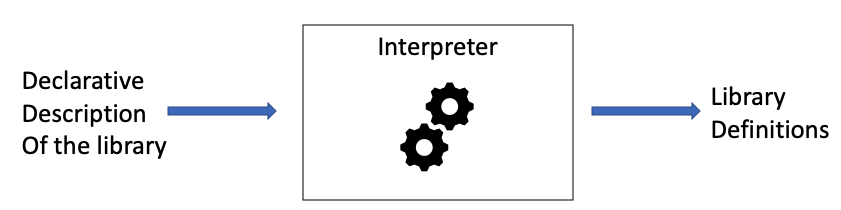
\includegraphics[scale=0.2]{figures/interpreter_small.png}
\end{figure}
\pause
\begin{itemize}
    \item Inspiration: Haskell  
\begin{onlyenv}<2>
    \begin{minted}[fontsize=\footnotesize]{haskell}
data List a = Nil | Cons a (List a) 
          deriving (Eq, Show, Ord, Read,
              -- by enabling some extensions 
                    Functor, Generic, Data,         
                    Foldable,Traversable, Lift)
    \end{minted}
    \vspace{0.5cm}
    \begin{minted}[fontsize=\footnotesize]{haskell}
data Point = Point { _x :: Double, _y :: Double }
makeLenses ''Point  
     \end{minted}
\end{onlyenv}     
\end{itemize}
\end{frame}

\begin{frame}[fragile]
\frametitle{Requirements}
\begin{enumerate}
\item A small language to represent theories without unnecessary details. 
\item Meta programs to manipulate these theories  
\item A type checker for the theories and constructions 
\item A large library of theories.
\end{enumerate}
\end{frame}

\begin{frame}[fragile]
\frametitle{Tog: Language and TypeChecker}
\begin{itemize}
    \item Dependently typed language 
    \begin{itemize}
        \item Martin-L\"{o}f type theory. 
    \end{itemize}
    \item Experimental language, in the style of Agda 
\end{itemize}
\begin{minted}[fontsize=\scriptsize]{Agda}
record Monoid (A : Set) : Set where
  constructor monoid
  field
   e  : A
   op : A -> A -> A
   lunit : {x : A} -> (op e x) == x
   runit : {x : A} -> (op x e) == x
   assoc : {x y z : A} -> 
     (op x (op y z)) == (op (op x y) z)
\end{minted}
\end{frame}

\begin{frame}[fragile]
\frametitle{Approach} 
\begin{figure}
    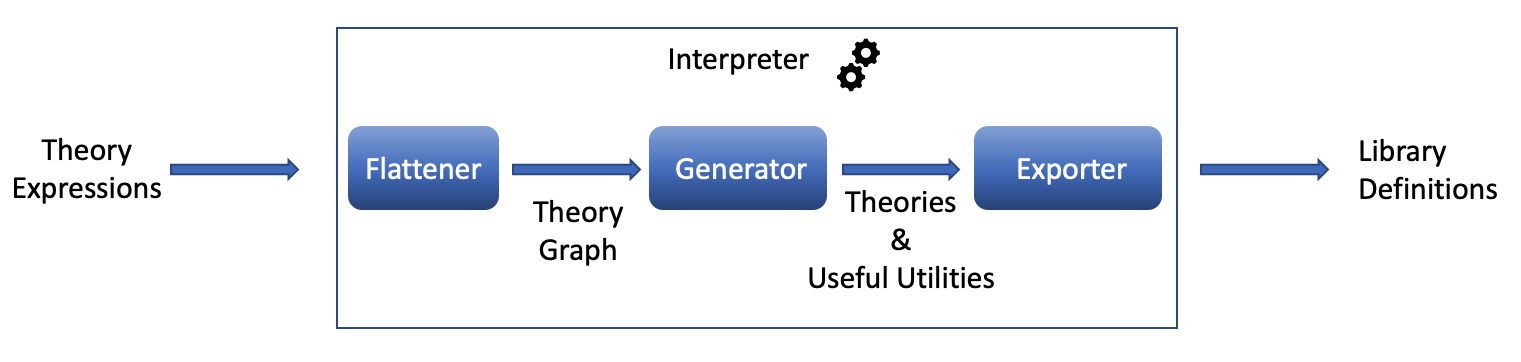
\includegraphics[scale=0.2]{figures/interpreter_detailed.png}
\end{figure}
\end{frame}

%\section{The Flattener}
\begin{frame}[fragile] 
\frametitle{The Flattener} 

%\centering{
\begin{center}
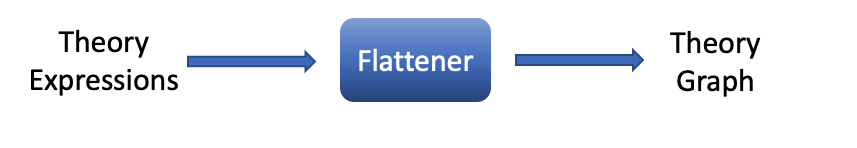
\includegraphics[scale=0.2]{figures/flattener.png}
\end{center}

\textcolor{Orange}{\textbf{Theory Graph}}



%\begin{figure}[h]
	\begin{tikzcd}[row sep=huge, column sep=scriptsize]
		&& & \verb|Pointed0| \arrow[dd,hook] & \\
		\verb|Carrier| \arrow[dd,hook] \arrow[rr,hook] & & \verb|Pointed| \arrow[ur,mapsto] & & \\ 
		& \verb|AddMagma| \arrow[rr,hook] \arrow[dd,hook]& & \verb|AddPointedMagma| 
		\arrow[rr,hook] 
		\arrow[dd,hook]& & 
		\verb|AddRightUnital|  \arrow[dd,hook]\\
		\verb|Magma| \arrow[ur,mapsto] \arrow[dd,hook]  & & 
		\verb|PointedMagma| \arrow[dd,hook] \arrow[ur,mapsto] \arrow[from=uu, crossing over] 
		\arrow[rr,hook,crossing over] \arrow[from=ll,hook, crossing over]
		& & \verb|RightUnital| \arrow[ur,mapsto] \\ 
		& \verb|AddSemigroup| \arrow[ddd,hook] & &\verb|AddLeftUnital| \arrow[rr,hook] &  & 
		\verb|AddUnital| \arrow[dddllll,hook] \\
		\verb|Semigroup|  \arrow[ddd,hook] \arrow[ur,mapsto]&  & \verb|LeftUnital| 
		\arrow[ur,mapsto] 
		\arrow[rr,hook,crossing over] &  & \verb|Unital| \arrow[dddllll,hook,crossing 
		over]\arrow[ur,mapsto] 
		\arrow[from=uu,hook,crossing over]& \\ 
		&&&& \\ 
		&  \verb|AddMonoid| &  &&\\ 
	 \verb|Monoid|  \arrow[ur,mapsto] && &&
	\end{tikzcd}
	\caption{Defining Monoid using tiny theories}
	\label{fig:cube_monoid}
%\end{figure}	

\end{frame}

\begin{frame}[fragile] 
\frametitle{The Flattener: Combinators} 
\textcolor{Orange}{\textbf{Theory Expressions}} \vspace{0.2cm}

\begin{overprint}
\onslide<1>
\begin{columns}
\begin{column}{0.45\textwidth}
\scriptsize{1. Extension}
\begin{minted}[fontsize=\scriptsize]{agda}
Semigroup  = extend Magma {assoc: ...}
\end{minted}
\end{column}
\begin{column}{0.45\textwidth}


{\scriptsize
  \begin{tikzcd}[row sep=2.0em, column sep=2.5em]
    \verb|Magma| \arrow[r,hook,blue] & \verb|Semigroup| 
  \end{tikzcd}
}
\end{column}
\end{columns}

\onslide<2>
\begin{columns}
\begin{column}{0.45\textwidth}
\scriptsize{1. Extension}
\begin{minted}[fontsize=\scriptsize]{agda}
Semigroup  = extend Magma {assoc: ...}
\end{minted}
\vspace{0.3cm}
\scriptsize{2. Rename}
\begin{minted}[fontsize=\scriptsize]{agda}
AdditiveMagma = rename Magma {op to +} 
\end{minted}
\end{column}
\begin{column}{0.45\textwidth}
{\scriptsize
  \begin{tikzcd}[row sep=2.0em, column sep=2.5em]
    \verb|Magma| \arrow[r,hook] \arrow[d,mapsto,blue] & \verb|Semigroup| & \\
    \verb|AdditiveMagma| & &
  \end{tikzcd}
}
\end{column}
\end{columns}

\onslide<3>
\begin{columns}
\begin{column}{0.45\textwidth}
\scriptsize{1. Extension}
\begin{minted}[fontsize=\scriptsize]{agda}
Semigroup  = extend Magma {assoc: ...}
\end{minted}
\vspace{0.3cm}
\scriptsize{2. Rename}
\begin{minted}[fontsize=\scriptsize]{agda}
AdditiveMagma = rename Magma {op to +} 
\end{minted}
\vspace{0.3cm}
\scriptsize{3. Combine}
\begin{minted}[escapeinside=~~,mathescape=true,fontsize=\scriptsize]{agda}
AdditiveSemigroup = 
  combine Semigroup {op to +} AdditiveMagma {} 
\end{minted}
\end{column}
\begin{column}{0.45\textwidth}
{\scriptsize
\begin{tikzcd}[row sep=2.0em, column sep=2.5em]
    \verb|Magma| \arrow[r,hook] \arrow[d,mapsto] \arrow[rd, blue] & \verb|Semigroup| \arrow[d,mapsto,blue]  \\
    \verb|AdditiveMagma| \arrow[r,hook,blue] & \verb|AdditiveSemigroup|
\end{tikzcd}
}
\end{column}
\end{columns}
\end{overprint}
\end{frame}


\begin{frame}[fragile]
\frametitle{The Flattener: Computing Pushouts}
 Pushouts are a $5$-ary operations: \hspace{1cm} 
 {\scriptsize
\begin{tikzcd}[row sep=2.0em, column sep=2.5em]
    \Gamma \arrow[r] \arrow[d]  & \Delta \\
    \Phi & 
\end{tikzcd}
}
\begin{itemize}
\item $3$ theories. 
\item $2$ arrows.
\end{itemize}
% \begin{itemize}
% \item $3$ theories 
% \item $2$ morphisms 
% \end{itemize}
 \pause 
 \vspace{0.5cm}
\begin{minted}[fontsize=\scriptsize]{agda}
combine AdditiveMonoid {} Group { ... } 
combine AdditiveMonoid {} MultMonoid {}  
\end{minted}
\vspace{0.5cm}
\begin{columns}
\begin{column}{0.45\textwidth}
{\scriptsize
\begin{tikzcd}[row sep=2.0em, column sep=2.5em]
    \verb|??| \arrow[r,hook] \arrow[d,mapsto]  & \verb|Group| \\
    \verb|AdditiveMonoid| & 
\end{tikzcd}
}
\end{column}
\begin{column}{0.45\textwidth}
{\scriptsize
\begin{tikzcd}[row sep=2.0em, column sep=2.5em]
    \verb|??| \arrow[r,hook] \arrow[d,mapsto]  & \verb|MultMonoid| \\
    \verb|AdditiveMonoid| & 
\end{tikzcd}
}
\end{column}
\end{columns} 
\pause 
\vspace{1cm}
\begin{minted}[escapeinside=~~,fontsize=\scriptsize]{agda}
combine AdditiveMonoid {} Group { ... } ~\textcolor{Blue}{over Monoid}~ 
combine AdditiveMonoid {} MultMonoid {} ~\textcolor{Blue}{over Carrier}~ 
\end{minted}
\end{frame}

\begin{frame}[fragile]
\frametitle{The Flattener} 
\begin{center}
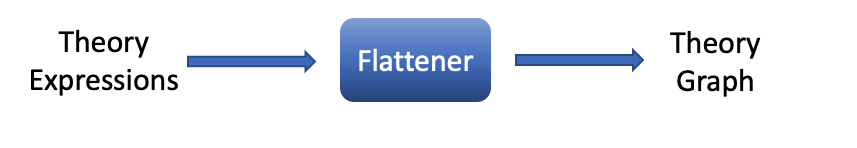
\includegraphics[scale=0.2]{figures/flattener.png}
\end{center}

\begin{overprint}
\begin{columns}
\begin{column}{0.45\textwidth}
\begin{minted}[fontsize=\scriptsize]{agda}
Pointed = extend Carrier {e : A}
Magma   = 
  extend Carrier {op : A -> A -> A}
Semigroup    = 
  extend Magma {assoc: ...}
PointedMagma = 
  combine Pointed {} Magma {} over Carrier
LeftUnital   = 
  extend PointedMagma { lunit_e : ... }
RightUnital  = 
  extend PointedMagma { runit_e : ... }
Unital = combine LeftUnital {} RightUnital {} 
         over PointedMagma
Monoid = combine Unital {} Semigroup {} over Magma
\end{minted}
\end{column}
\begin{column}{0.45\textwidth}



{\tiny
  \begin{tikzcd}[row sep=2.0em, column sep=2.5em]
    \verb|Carrier| \arrow[d,hook] \arrow[r,hook] \arrow[dr,hook]& \verb|Pointed| \arrow[d,hook]& \\
    \verb|Magma| \arrow[d,hook] \arrow[r,hook] & 
    \verb|PointedMagma|  \arrow[d,hook] \arrow[rr,hook] \arrow[drr,hook]
    & & \verb|RightUnital|  \arrow[d,hook]\\
    \verb|Semigroup| \arrow[rd,hook] & \verb|LeftUnital| \arrow[rr,hook] & &\verb|Unital| \arrow[dll,hook] & \\
   & \verb|Monoid|  & &&
  \end{tikzcd}
}
\end{column}
\end{columns}
\end{overprint}
\end{frame}

\begin{frame}[fragile] 
%\begin{adjustbox}{width=0.5\textwidth,center}
%\scalebox{0.7}{
\parbox{\linewidth}{
\begin{tiny}
Empty, Carrier, Pointed, UnaryOperation, PointedUnarySystem, FixedPoint, Magma, 
AdditiveMagma, MultMagma, PointedMagma, Involution, UnaryDistributes, UnaryAntiDistribution, IdempotentUnary, InvolutiveMagma, LeftInverseMagma, RightInverseMagma, IdempotentMagma, IdempotentAdditiveMagma, Pointed0Magma, PointedPlusMagma, AdditivePointedMagma, Pointed1Magma, PointedTimesMagma, MultPointedMagma, CommutativeMagma, CommutativeAdditiveMagma, CommutativePointedMagma, AntiAbsorbent, SteinerMagma, Squag, PointedSteinerMagma, Sloop, LeftDistributiveMagma, RightDistributiveMagma, Unital, LeftBiMagma, RightBiMagma, QuasiGroup,
MoufangLaw, MoufangQuasiGroup, Loop, MoufangIdentity, MoufangLoop, Shelf, LeftBinaryInverse, RightBinaryInverse, BinaryInverse, Rack, Spindle, Quandle, RightSelfInverse, Semigroup, AdditiveSemigroup, CommutativeSemigroup, MultCommutativeSemigroup, CancellativeSemigroup, InvolutivePointedSemigroup, Band, MiddleAbsorption, MiddleCommute, RectangularBand, NormalBand, RightMonoid, LeftMonoid, PointedSemigroup, AdditivePointedSemigroup, AdditiveUnital, MultPointedSemigroup, Monoid, AdditiveMonoid, DoubleMonoid, CommutativeMonoid, CancellativeMonoid, CancellativeCommutativeMonoid, Zero, AdditiveCommutativeMonoid, BooleanGroup, InverseUnaryOperation, Inverse, PseudoInverse, PseudoInvolution, RegularSemigroup, QuasiInverse, Group, AdditiveGroup, CommutativeGroup, MultGroup, AbelianGroup, AbelianAdditiveGroup, RingoidSig, LeftRingoid, RightRingoid, Ringoid, NonassociativeRing, AndDeMorgan, OrDeMorgran, DualDeMorgan, AssociativeLeftRingoid, LeftPreSemiring, AssociativeRightRingoid, RightPreSemiring, PreSemiring, AssocPlusRingoid, AssocTimesRingoid, NearSemiring, NearRing, SemiRng, Rng, SemiRngWithUnit, Semiring, Ring, CommutativeRing, BooleanRing, IdempotentSemiRng, IdempotentSemiring, InvolutiveFixes, InvolutiveFixedPoint, InvolutiveRingoid, InvolutiveRing, JacobianIdentity, AntiCommutativeRing, LieRing, MeetSemilattice, MultMeetSemilattice, BoundedMeetSemilattice, JoinSemilattice, BoundedJoinSemilattice, DualSemilattices, LeftAbsorption, LeftAbsorptionOp, Absorption, Lattice, Modularity, ModularLattice, DistributiveLattice, BoundedJoinLattice, BoundedMeetLattice, BoundedLattice, BoundedModularLattice, BoundedDistributiveLattice,
\end{tiny}}
%\end{adjustbox}
\end{frame}

%\section{The Generator}
\begin{frame}[fragile]
\frametitle{The Generator}
\begin{center}
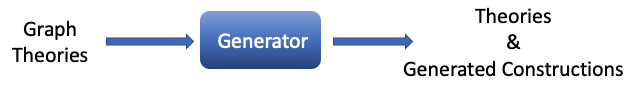
\includegraphics[scale=0.25]{figures/generator.png}
\end{center}
\pause
\begin{itemize}
\item Uni-sorted equational theory: 
$\Gamma = (\mathcal{S},\mathcal{F},\mathcal{E})$
\vspace{0.2cm}
\begin{minted}[escapeinside=||,mathescape=true,fontsize=\scriptsize]{haskell}
data EqTheory = EqTheory  {
  name        :: Name_   ,
  sort        :: Constr  ,  -- the carrier $\mathcal{S}$
  funcTypes   :: [Constr],  -- function symbols $\mathcal{F}$
  axioms      :: [Constr],  -- equations $\mathcal{E}$
  waist       :: Int        -- the number of parameters
}  
\end{minted}
% |\tikzmark{ssort}|
\begin{comment}
\begin{minted}[escapeinside=||,mathescape=true,fontsize=\scriptsize]{text}
record |\fcolorbox{blue}{white}{Monoid \fcolorbox{red}{white}{(A : Set)}}| : Set where -- waist = 1  
  e  : A 
  op : A |$\to$| A |$\to$| A 
  lunit : ...
  runit : ... 
  assoc : ...
\end{minted} 
\end{comment}
\pause
\item Instance of a theory:  
\begin{minted}[escapeinside=||,mathescape=true,fontsize=\scriptsize]{haskell}
type EqInstance = (Name|\_|,[Binding],Expr) 
\end{minted}
\scriptsize{Example:} 
\begin{minted}[escapeinside=||,mathescape=true,fontsize=\scriptsize]{text}
          {A : Set} |$\to$| M : Monoid A   
\end{minted}
%\begin{minted}[escapeinside=||,mathescape=true,fontsize=\scriptsize]{text}
%type EqInstance = (|\fcolorbox{blue}{white}{Na\tikzmark{name}me\_}|,|\fcolorbox{red}{white}{[Bin\tikzmark{binds}ding]}|,|\fcolorbox{green}{white}{Ex\tikzmark{expr}pr}|) 
%|\fcolorbox{red}{white}{{A : Set}}| |$\to$| |\fcolorbox{blue}{white}{M}| : |\fcolorbox{green}{white}{Monoid A}|   
%\end{minted}
\end{itemize}
%\begin{tikzpicture}[node distance=2cm]
    \node(NodeName1){
\begin{lstlisting}[basicstyle=\footnotesize, escapeinside=~~]
record ~\fcolorbox{blue}{white}{Monoid \fcolorbox{red}{white}{(A : Set)}}~
      : Set where 
  e  : ~\fcolorbox{red}{white}{A}~ 
  op : ~\fcolorbox{red}{white}{A}~ -> ~\fcolorbox{red}{white}{A}~ -> ~\fcolorbox{red}{white}{A}~ 
  lunit : ...
  runit : ... 
  assoc : ...
\end{lstlisting} 
};
\node(NodeName2) [right=of NodeName1] {  % added position of second box
\begin{lstlisting}[basicstyle=\footnotesize, escapeinside=~~]
record Hom ~\fcolorbox{red}{white}{\{A1 A2 : Set\}}~ 
       ~\fcolorbox{blue}{white}{(M1 : Monoid A1) (M2 : Monoid A2)}~
       : Set where 
  hom : ~\fcolorbox{red}{white}{A1}~ -> ~\fcolorbox{red}{white}{A2}~ 
  pres-e : hom ~\fcolorbox{green}{white}{(e M1)}~ = ~\fcolorbox{green}{white}{e M2}~ 
  pres-op : {x1 x2 : A1} -> 
    hom (~\fcolorbox{green}{white}{(op M1) x1 x2}~) = 
    ~\fcolorbox{green}{white}{(op M2) (hom x1) (hom x2)} 
\end{lstlisting} };  



%\draw[red, line width=0.5mm,-{Triangle[angle=60:0.5pt 3]}] (NodeName1) -- (NodeName2);
%\draw[blue, line width=1mm,-{Triangle[angle=60:1pt 3]}] (NodeName1) -- (NodeName3);
\end{tikzpicture}

\begin{comment}
\begin{minted}[fontsize=\scriptsize,escapeinside=||]{Agda}
record Monoid (A : Set) (e : A) : Set where 
  constructor monoid
  field
   op : A -> A -> A
   lunit : {x : A} -> (op e x) == x
   runit : {x : A} -> (op x e) == x
   assoc : {x y z : A} -> 
     op x (op y z) == op (op x y) z
\end{minted}
\end{comment}

%\begin{tikzpicture}[remember picture]
%\draw[overlay, ->] (pic cs:name) -- (pic cs:nm); %to[bend right]
%\draw[overlay, ->] (pic cs:binds) -- (pic cs:bi); %, line width=5pt, red
%\draw[overlay, ->] (pic cs:expr) -- (pic cs:ex);
%\end{tikzpicture}
\end{frame}

\begin{frame}[fragile] 
\frametitle{Constructions for Free!} 
\begin{tikzpicture}[node distance=2cm]
    \node(NodeName1){
\begin{lstlisting}[basicstyle=\footnotesize, escapeinside=~~]
record ~\fcolorbox{blue}{white}{Monoid \fcolorbox{red}{white}{(A : Set)}}~
      : Set where 
  e  : ~\fcolorbox{red}{white}{A}~ 
  op : ~\fcolorbox{red}{white}{A}~ -> ~\fcolorbox{red}{white}{A}~ -> ~\fcolorbox{red}{white}{A}~ 
  lunit : ...
  runit : ... 
  assoc : ...
\end{lstlisting} 
};
\node(NodeName2) [right=of NodeName1] {  % added position of second box
\begin{lstlisting}[basicstyle=\footnotesize, escapeinside=~~]
record Hom ~\fcolorbox{red}{white}{\{A1 A2 : Set\}}~ 
       ~\fcolorbox{blue}{white}{(M1 : Monoid A1) (M2 : Monoid A2)}~
       : Set where 
  hom : ~\fcolorbox{red}{white}{A1}~ -> ~\fcolorbox{red}{white}{A2}~ 
  pres-e : hom ~\fcolorbox{green}{white}{(e M1)}~ = ~\fcolorbox{green}{white}{e M2}~ 
  pres-op : {x1 x2 : A1} -> 
    hom (~\fcolorbox{green}{white}{(op M1) x1 x2}~) = 
    ~\fcolorbox{green}{white}{(op M2) (hom x1) (hom x2)} 
\end{lstlisting} };  



%\draw[red, line width=0.5mm,-{Triangle[angle=60:0.5pt 3]}] (NodeName1) -- (NodeName2);
%\draw[blue, line width=1mm,-{Triangle[angle=60:1pt 3]}] (NodeName1) -- (NodeName3);
\end{tikzpicture}

\begin{overprint}
\onslide<1>
\begin{minted}[escapeinside=||,mathescape=true,fontsize=\scriptsize]{haskell} 
homomorphism :: Eq.EqTheory -> Decl
homomorphism thry =
  let nm = "Hom" 
     i1@(|\fcolorbox{blue}{white}{n1},\fcolorbox{red}{white}{b1},\fcolorbox{green}{white}{e1}|) = Eq.eqInstance thry (Just 1)
      i2@(n2,b2,e2) = Eq.eqInstance thry (Just 2)
      fnc    = homFunc thry i1 i2
      axioms = map (presAxiom thry i1 i2 fnc) (thry ^. Eq.funcTypes)  
  in Record (mkName nm)
   (mkParams |$\$$| |\fcolorbox{red}{white}{b1 ++ b2 ++}|
               map (|$\backslash$|(n,e) -> Bind [mkArg n] e) [(|\fcolorbox{blue}{white}{n1}|,|\fcolorbox{green}{white}{e1}|),(|\fcolorbox{blue}{white}{n2}|,|\fcolorbox{green}{white}{e2}|)])}
   (RecordDeclDef setType (mkName |$\$$| nm ++ "C") (mkField |$\$$| fnc : axioms))
\end{minted} 
\end{overprint}
\end{frame}

\begin{frame}[fragile] 
\frametitle{Constructions for Free!} 
\begin{figure}
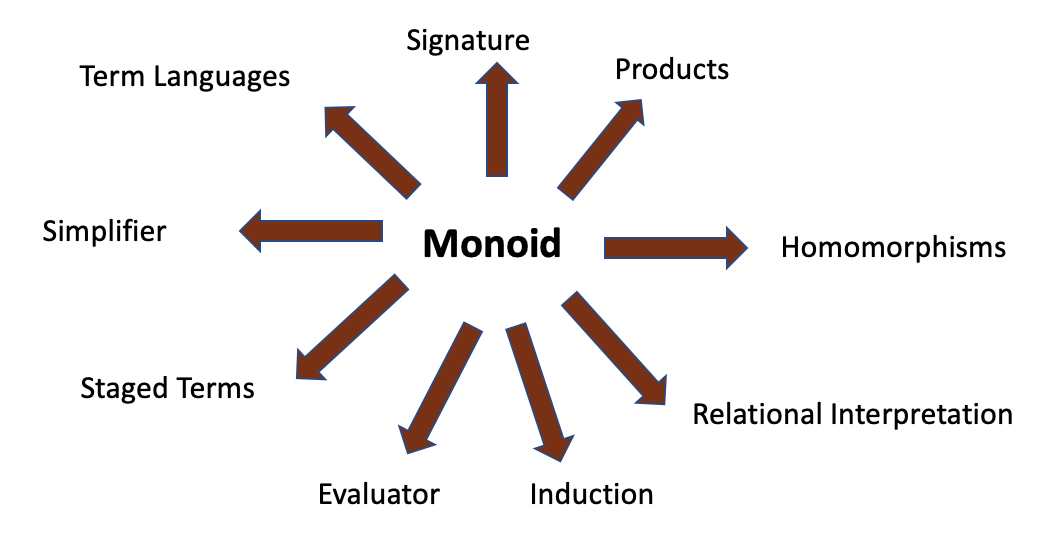
\includegraphics[scale=0.25]{figures/monoid_generation2.png}
\end{figure}
\scriptsize
monomorphism, epimorphism, endomorphism, isomorphism, automorphism, kernel of a morphism, composition of morphisms, quotient algebra, sub-theory, trivial sub-theory, parse trees, equivalence of terms, ...   
\end{frame}

%\section{The Exporter}

\begin{comment}
\begin{frame}[fragile] 
\frametitle{The Exporter} 
\begin{minted}[escapeinside=||,mathescape=true,fontsize=\scriptsize]{agda} 
data MonTerm  (n : Nat) (A : Set) : Set where 
  v : Fin n |$\to$| MonTerm n A 
  sing : A |$\to$| MonTerm n A 
  op : MonTerm n A |$\to$| MonTerm n A |$\to$| MonTerm n A 
  e : MonTerm n A 
\end{minted}
\begin{minted}[escapeinside=~~,mathescape=true,fontsize=\scriptsize]{lean} 
inductive MonTerm  (n : Nat) (A : Type) : Type 
  | v : Fin n ~$\to$~ MonTerm
  | sing : A ~$\to$~ MonTerm
  | op : MonTerm ~$\to$~ MonTerm ~$\to$~ MonTerm 
  | e  : MonTerm
open MonTerm   
\end{minted}
\begin{minted}[escapeinside=~~,mathescape=true,fontsize=\scriptsize]{lean} 
def evalOp   {A : Type} {n : ~$\mathbb{N}$~}  : ((Monoid A) ~$\to$~ ((vector A n) ~$\to$~ ((OpMonoidTerm2 n A) ~$\to$~ A))) 
  | Mo vars (v2 x1) := (nth vars x1)  
  | Mo vars (sing2 x1) := x1  
  | Mo vars (opOL2 x1 x2) := ((op Mo) (evalOp Mo vars x1) (evalOp Mo vars x2))  
  | Mo vars eOL2 := (e Mo)  
\end{minted}
\end{frame}
\end{comment}

\begin{frame}[fragile] 
\frametitle{The Exporter} 
\begin{center}

\includegraphics[scale=0.25]{figures/exporter.png}
\end{center} 
\end{frame}

\begin{frame}[fragile] 
\frametitle{The Exporter} 
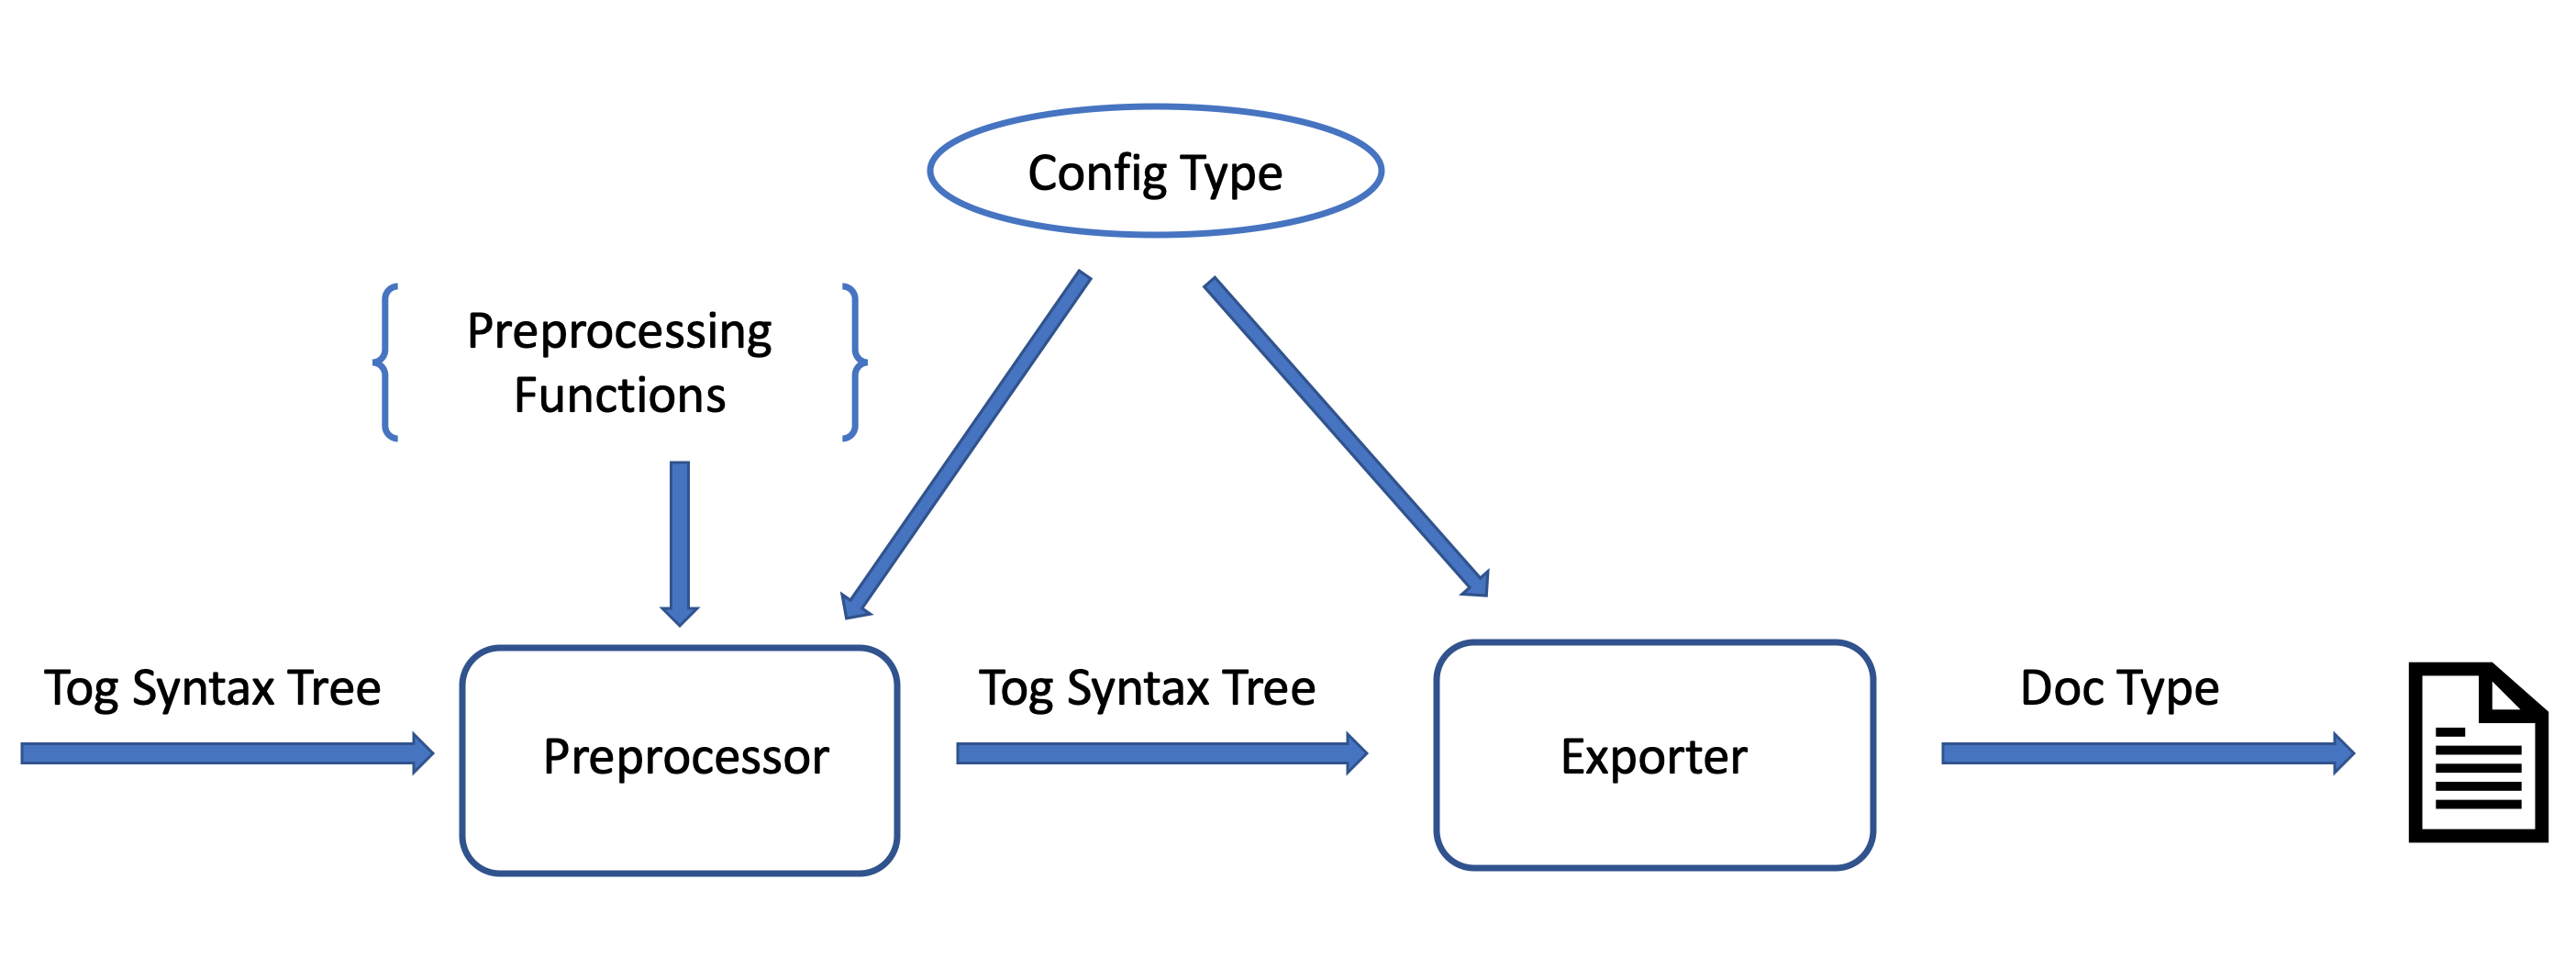
\includegraphics[scale=0.2]{../figures/exporter_arch.png}
\begin{overprint}
\onslide<1>
\textbf{Preprocessor}
\begin{itemize}
\item Universes 
\item Prelude definitions 
\item Non-linear pattern matching 
\item Functions as constructors
\item Names misalignment  
\end{itemize}
\onslide<2>
\textbf{Exporter}
\begin{minted}[fontsize=\scriptsize]{haskell} 
class Export a where
  export :: Config -> a -> Doc
\end{minted} 
\lstmath{Config}: captures language-specific information. 
\end{overprint}
\end{frame}

\begin{frame}[fragile] 
\frametitle{Results}
Starting with \textbf{\textcolor{Orange}{227}} theory expressions:
\begin{itemize}
\item \textcolor{Orange}{\textbf{5092}} library definitions. 
\item \textcolor{Orange}{\textbf{32,459}} lines of code. 
\item Exported to \textcolor{Orange}{\textbf{Lean}}, \textcolor{Orange}{\textbf{Agda}} (flat and predicate style theories).
\pause
\item Average time: \\ \vspace{0.25cm}
\begin{center}
\begin{adjustbox}{width=0.4\columnwidth}
\begin{tabular}{| c | c |}\hline
Flattener & 5.17 s \\ \hline
Generator & 2.7 s \\ \hline
Exporter & 9.1 us \\ \hline
Type-checking & 28 mins \\ \hline
\end{tabular}
\end{adjustbox}
\end{center}
\end{itemize}
\end{frame}

%\section{Conclusion and Future Work}
\begin{frame}[fragile] 
\frametitle{Future Work}
\begin{itemize}
\item Generalizing the approach to \textcolor{Orange}{\textbf{generalized algebraic theories}}.

\vspace{0.5cm}
\item Proof assistants as \textcolor{Orange}{\textbf{program families}}. 
\begin{itemize}
\item better understanding how design decisions affect theory presentations 
\item staged exporter to multiple proof assistants 
\end{itemize}

\vspace{0.5cm}
\item a \textcolor{Orange}{\textbf{DSL}} for library development. 
\vspace{0.2cm}
\begin{minted}[escapeinside=||,mathescape,fontsize=\scriptsize]{Haskell}
Monoid = combine Unital and Semigroup over Magma
         generate Homomorphism, OpenTerms, Simplifier
         using (waist=1,eq="=")
         export_to lean
\end{minted}
\end{itemize}
\end{frame} 

\begin{frame}[fragile] 
\frametitle{Conclusion} 
Summary of Contributions: 
\begin{itemize}
\item Highlighted the redundancy in libraries formalizing the algebraic hierarchy.
\item Built a library of $227$ theories describing the algebraic hierarchy using theory combinators.
\item Compiled a list of structures that can be generated from theory presentations.
\item Generated some of these constructions in Tog, a small implementation of a dependently typed language.
\item Exported this implementation to Agda and Lean.
\end{itemize}
\end{frame}

\end{document}
